
\chapter{Contextualizaci\'on}

\section{Robots de servicio}

La Federaci\'on Internacional de Rob\'otica (IFR)\cite{IFR} define \textit{robot} como:
\begin{quotation}
``Un mecanismo actuado y programable en dos o m\'as ejes y con un cierto grado de autonom\'ia, que se mueve en su entorno para realizar tareas previstas. En este contexto, autonom\'ia se refiere a la habilidad de realizar tareas previstas, basado en el estado actual y lo sensado, sin intervenci\'on humana.''
\end{quotation}

Asimismo, la IFR define un \textit{robot de servicio} como un robot ``que realiza tareas \'utiles para humanos o equipamiento, excluyendo aplicaciones de automatizaci\'on industrial''. As\'i, un robot de servicio debe trabajar en ambientes no controlados y con la autonom\'ia suficiente que le permita llevar a cabo su cometido. Generalmente, la rob\'otica de servicio se enfoca en asistir a los seres humanos en tareas repetitivas y comunes.

Seg\'un su \'area de aplicaci\'on, un rob\'ot de servicio se clasifica en \textit{de uso personal} o \textit{de uso profesional}. Los primeros son utilizados en ambientes no comerciales y por personas comunes; como por ejemplo, un robot sirviente o una silla de ruedas aut\'onoma. Un robot de servicio profesional se utiliza en ambientes comerciales, usualmente operados por alguien entrenado; un ejemplo son los robots de entrega de paquetes o para cirug\'ia.


\subsection{Robots Dom\'esticos}

Seg\'un la recopilaci\'on de datos realizada por la IFR durante el 2016, este tipo de robots es utilizado en las siguientes \'areas:
\begin{itemize}[topsep=0pt]
\setlength\itemsep{0.2em}
\item Tareas dom\'esticas: De compa\~nia, asistencia, limpieza, cuidado del hogar.
\item Entretenimiento: Juguetes, comunicaci\'on, educaci\'on e investigaci\'on.
\item Asistencia a ancianos y discapacitados: Sillas rob\'oticas y robots para cuidar personas.
\item Transporte.
\item Seguridad y vigilancia.
\item Otros que no caen en las categor\'ias anteriores.
\end{itemize}
\bigskip

El foco de este trabajo son los robots de servicio personales, dedicados a tareas dom\'esticas, clasificaci\'on a la que en  adelante se referir\'a como \textit{Robots Dom\'esticos}.

Para entender el alcance del trabajo, en cuanto a qu\'e es lo que se espera del sistema, a continuaci\'on se listan algunas capacidades de los robots dom\'esticos. Un robot de compa\~nia y asistencia tiene, pero no se limita a las siguientes tareas:
\begin{itemize}[topsep=0pt]
\setlength\itemsep{0.2em}
\item Interacci\'on amistosa con humanos.
\item Ayudar a recordar y organizar tareas.
\item Cooperar con la realizaci\'on de un procedimiento.
\item Guiar y seguir a personas.
\item Recordar informaci\'on y entidades.
\end{itemize}
\bigskip

Algunas tareas que robots dom\'esticos de tipo mayordomo deben ejecutar son:
\begin{itemize}[topsep=0pt]
\setlength\itemsep{0.2em}
\item Ofrecer comida y bebestibles.
\item Preparaci\'on de comida.
\item Ordenar y limpiar el hogar.
\end{itemize}
\bigskip


\section{Memoria Humana}

La memoria es un elemento fundamental para los humanos en su d\'ia a d\'ia, y es parte integral de su existencia. Permite recordar qui\'en, qu\'e, c\'omo, d\'onde y cu\'ando. En t\'erminos psicol\'ogicos, es la habilidad para para codificar, almacenar y luego obtener informaci\'on sobre eventos pasados en el cerebro. Los pensamientos son parte de la memoria de corto plazo, mientras que eventos pasados son almacenados en una memoria de largo plazo. Existen muchos estudios en el \'area de la psicolog\'ia cognitiva con diversas descripciones y modelos te\'oricos de cada tipo de memoria\cite{Vijayakumar2014}.

Desde el punto de vista de la informaci\'on procesada, la memoria es vista como una facultad humana consistente en procesos para el manejo de informaci\'on. Los 3 componentes principales son:

\begin{itemize}
\item Codificaci\'on: En este paso, se adquiere nueva informaci\'on desde los sentidos humanos. Los datos son convertidos a un formato que pueda ser almacenado en la estructura cerebral correspondiente.
\item Almacenamiento: Consiste en la creaci\'on de registros permanentes de informaci\'on. Es un proceso pasivo, de continuo procesamiento para clasificar datos nuevos y los ya existentes en el cerebro.
\item Adquisici\'on: Hace referencia al acceso de datos almacenados. El proceso se realiza en el momento, para obtener una reconstrucci\'on aproximada de la informaci\'on, a partir de elementos repartidos en distintas partes del cerebro.
\end{itemize}


La memoria puede ser dividida en m\'ultiples sistemas de independientes, con funcionalidades bien definidas y sustentados por distintas estructuras cerebrales. La primera diferenciaci\'on define dos tipos de memoria: la memoria de corto y la de largo plazo, STM (Short-Term Memory) y LTM (Long-Term Memory), por sus siglas en ingl\'es. En el diagrama de la figura \ref{img:human_memory} se muestra una separaci\'on cl\'asica utilizada en el \'area de las ciencias cognitivas\cite{Eichenbaum:2008}, explicada en las siguientes subsecciones.

\begin{figure}[H]
\centering
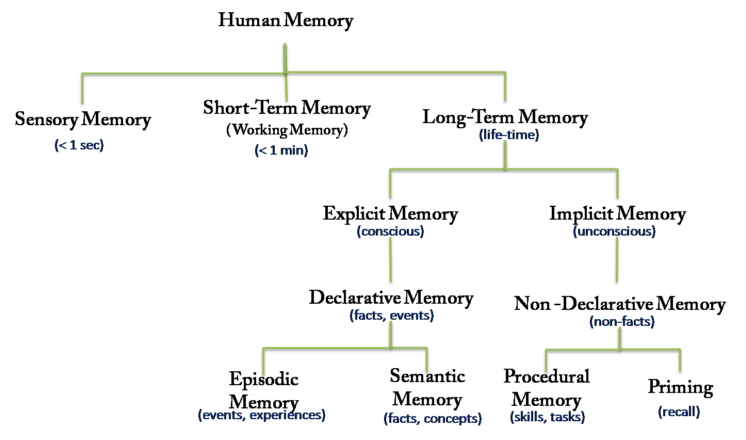
\includegraphics[width=0.8\textwidth]{./figures/diagrama_memoria.png}
\caption{\small Clasificaciones de la memoria humana. Obtenido de \cite{Vijayakumar2014}.}
\label{img:human_memory}
\end{figure}

% Sobre el estudio de la memoria.. origenes.. Tulving 

\subsection{Memoria de Corto Plazo}

En el \'ambito cognitivo, la STM se refiere a la habilidad de estar atento, recopilar informaci\'on  y memorias, para luego utilizarlas dentro de un corto periodo de tiempo. Es responsable de almacenar informaci\'on constantemente y de decidir que parte ser\'a transferida a la memoria de largo plazo. El t\'ermino de \textit{Memoria de Trabajo} suele ser utilizado de manera intercambiable con el de STM. Adem\'as, suele ser agrupada con otro tipo de memoria, llamada \textit{Sensorial}.

La STM se caracteriza por manejar informaci\'on muy detallada, ser de poca capacidad y permitir un r\'apido acceso a estos datos. Permite recordar r\'apidamente y con gran detalle, experiencias ocurridas hace pocos segundos, pero con dificultad creciente a medida que avanza el tiempo.

Se sustenta principalmente en la corteza prefrontal del cerebro. Algunos estudios han mostrado que las neuronas involucradas son capaces de mantener informaci\'on relevante de corto plazo, la que es combinada con informaci\'on sensorial entrante y \'areas que manejan la toma de decisiones. %(Miller, 2000).
En los humanos, esta \'area presenta gran activaci\'on durante procesos de codificaci\'on, acceso y manipulaci\'on de memorias. %(Postle, 2006). 


\subsection{Memoria de Largo Plazo}

, mientras que la LTM maneja mucha informaci\'on sobre experiencias y entidades, es menos detallada y de acceso m\'as lento\cite{Eichenbaum:2008}.

Sobre semantica... la gente no olvida, sin oque solo debilita links


Memoria explicita (conciente)
declarativa: hechos eventos .. . episodica, semantica


memoria implicita (inconsciente)

no declarativa> procedural, priming

descripcion general...

\subsection{Funcionalidades}

Semantic Memory “Is a network of associations and concepts that underlies our basic knowledge of the
worldword meanings, categories, facts, and propositions, and the like” [15, p. 150]. This memory stores world knowledge like that a table typically has four legs. It is accessed by a human if he can say “I know”.
• Procedural Memory “Is a kind of bodily memory. It is memory for habitual motor skills, or, more generally,
perceptuomotor or ideomotor skill” [15, p. 156]. Knowl- edge about periodically tasks like running or swimming is stored here.
• Episodic Memory “Involves the literal reexperiencing of past events–the bringing back to awareness of previous
experiential episodes” [15, p. 160]. Here, the personal experiences like having been in school are stored. A human accesses this memory if he can say “I remember”.


La LTM se puede dividir en expl\'icita (consciente) e impl\'icita (inconsciente). La primera almacena datos epis\'odicos, pudiendo responder las preguntas ``Qu\'e'', ``D\'onde'' y ``Cu\'ando'', datos sem\'anticos, que modelan hechos y conceptos como el lenguaje o personas, y tambi\'en, las conexiones entre ambas submemorias. La memoria impl\'icita codifica habilidades, h\'abitos y preferencias.



La memoria emocional es una forma de memoria impl\'icita que genera reacciones emocionales y sentimientos. Seg\'un los est\'imulos a los que se enfrente, permite modular el proceso de consolidaci\'on de la STM en LTM, modificando el nivel de relevancia de los eventos, pudiendo generar memorias muy fuertes y h\'abitos arraigados. Ejemplos de esto son los flashbacks y las memorias asociadas a eventos importantes.


\subsection{Procesos}

Existen procesos de consolidaci\'on y deterioro de la memoria que est\'an constantemente en funcionamiento. La consolidaci\'on requiere un est\'imulo relevante, sumado al proceso de almacenamiento, lo que genera conexiones entre la memoria epis\'odica y la respectiva zona sem\'antica. En caso de haber experiencias repetidas, las conexiones se fortalecen. El deterioro de la memoria es un proceso que degenera las conexiones entre ambas formas de memorias expl\'icitas.





\section{Memoria y rob\'otica}

requerimientos para interaccion humana y tareas que debe desarrollar un robot de servicio.
%\subsection{Interacci\'on Humano-Computador}
%
%\subsection{Interacci\'on con el entorno}

sobre importancia de la memoria en un sistema robotico!!!
... blabla util \cite{Vijayakumar2014}
... como memoria ayuda a mejorar desempeno en tareas \cite{Salgado2012}
... mas al respecto \cite{Ho2009}
... casos de uso e inferencia \cite{Vijayakumar2014}


diagramas
... memoria humana \cite{Vijayakumar2014}
... memoria humana LTM \cite{Stachowicz2012}
... consolidacion y olvido \cite{Deutsch2008}

Punto de vista de las ciencias cognitivas
... agregar!!! o mover a la memoria humana
... referencias a psicoanalisis \cite{Deutsch2008}

Sobre casos quie no son human like...
- algunos solo base de datos y recordar todo
- deep neural network... \cite{KimMinJoo2016}


Muchos intentar basarse en bla...


Relacion memoria humana con robotica.
... habilidades y PM \cite{Salgado2012} ... CRAM
... datos y semantica
... sobre importancia del sueno y postprocesamiento \cite{Kelley2014}
 ... E LTM no solo responde que donde y cuando.. necesita perspectiva \cite{Stachowicz2012}
... S Memory.. se abstrae de perspecttiva y cosas situacionales \cite{Stachowicz2012}
... defs de memoria \cite{Deutsch2008}
... definiciones de procesos cognitivos: \cite{Deutsch2008}
 
 
Existen los siguientes modelos
- algunos solo procuran desarrollar reglas sobre como actualizar los pesos de aprendizaje
- dejar de aprender (sorprenderse al ser mayor)
... modelo probabilistico para consolidar y decaer \cite{Dodd2005}
... olvidar cosas.. si no se implementa, entonces la busqueda de informacion seria cada vez mas compleja. \cite{Deutsch2008}
... modelo capaz de adaptarse a m\'as robots \cite{Ho2009}
... modelo de contexto \cite{Sanchez:2015} FELIX

sobre el diseno..
... que recordar y cuando \cite{Kasap2010}
... conflicto etico de almacenar datos de usuarios \cite{Ho2009}
... aspectos de diseno \cite{Ho2009}
... propiedades de LTM \cite{Jockel2008}
... requerimientos de LTM \cite{Vijayakumar2014}
... requerimientos E LTM \cite{Stachowicz2012}
... 11 req. ELTM \cite{Stachowicz2012}
... sobre importancia del sueno y postprocesamiento \cite{Kelley2014}
... diseno explicado de SONIA en RDF \cite{Vijayakumar2014}
... definir contenido de QWHAT \cite{Stachowicz2012}

Existen los siguientes frameworks, modelos
- procedural y CRAM \cite{Winkler2014}
... ISAC \cite{Dodd2005}
... MINERVA, LIDA, Neuronal,M SMRTI \cite{Jockel2008}
... deficiencias de ISAC, EPIROME, \cite{Stachowicz2012}
... sobre Tecuci, ISAC, SOAR y Ho \cite{Deutsch2008}

Existen las siguientes reglas generales
.. definicion de episodio \cite{Dodd2005}
.. reglas de consolidacion \cite{Dodd2005}


sobre memoria emocional y mapeo al robot
.. emotion Engine \cite{Kasap2010}
.. mapeo por dolor. teoria de haikonen y otros \cite{Dodd2005}
... refs sobre emociones \cite{Deutsch2008}
.. emociones modulan el bla \cite{Deutsch2008}

sobre inferencia y mapeo al robot
.. sobre importancia del sueno y postprocesamiento \cite{Kelley2014}

Resumen de dificultades ... diagrama o tabla.



Considerar unificaci\'on de informaci\'on.. que pasa si almaceno obj1 y obj2, pero luego aprendo que son el mismo?



\section{Componentes de software}

La implementaci\'on de un sistema de memoria ro\'otica asume que muchos sistemas y capacidades de un robot est\'an disponibles. Entonces, se requiere del uso de variados frameworks y librer\'ias que permiten comunicarse con el robot y acceder a los datos de inter\'es que se desea recordar. A continuaci\'on se explican los componentes de software relevantes para el trabajo.

\subsection{ROS}

Los sistemas rob\'oticos actuales son cada vez m\'as complejos. Deben lidiar con muchos componentes tanto de hardware como de software y su interacci\'on, de una forma eficaz y que no entorpezca el desarrollo. Muchas tareas de control requieren altas frecuencias de funcionamiento, as\'i como la sincronizaci\'on y comunicaci\'on entre los diversos m\'odulos. Por lo tanto, el c\'omo se unen los subsistemas en una aplicaci\'on rob\'otica es una tarea dif\'icil.

ROS\cite{ROS:2009}, acr\'onimo para Robot Operating System, es un proyecto que funciona como middleware para aplicaciones rob\'oticas, y permite resolver el problema de la comunicaci\'on entre procesos. Es una colecci\'on de herramientas, librer\'ias y convenciones que buscan simplificar la tarea de crear comportamientos rob\'oticos complejos y robustos, sin importar la plataforma rob\'otica.

Fue originalmente creado por la empresa WillowGarage en el 2008, y mantenido actualmente por la Open Source Robotics Foundation (OSRF). Existe un ecosistema ROS, mantenido por la comunidad, y con cientos de m\'odulos de software con soluciones a problemas espec\'ificos, los que pueden interconectarse para construir comportamientos m\'as complejos. Por lo anterior, su uso se ha convertido en una pr\'actica mundial, siendo adoptado incluso en soluciones industriales.

\todo[inline]{M\'as informaci\'on sobre ROS. Lo que sea relevante para la implementaci\'on y el dise\~no}

%\subsubsection{Nodo}
%
%Mensajes y master
%
%\subsubsection{T\'opicos}
%
%\subsubsection{Servicios}
%
%\subsubsection{Servidor de par\'ametros}
%
%\subsubsection{Launch}

%\subsubsection{Herramientas}

%\subsubsection{Actionlib}


%\subsection{SMACH}

\todo[inline]{Sobre SMACH Ser\'a utilizado para la demo.}


\subsection{UChile ROS Framework}

UChile ROS Framework (URF) hace referencia al sistema de software desarrollado en el laboratorio de rob\'otica del Departamento de Ingenier\'ia El\'ectrica de la Universidad de Chile, para sus robots de servicio. El sistema cuenta con 10 a\~nos de desarrollo y est\'a orientado a cumplir los requisitos de la competencia Robocup en su categor\'ia @Home.

URF est\'a construido sobre ROS y en una estructura de 4 capas. La primera capa contiene todas las dependencias del sistema, ya sean de ROS o no; Es la \'unica capa donde que contiene c\'odigo externo. Sobre ella, se monta una capa ROS de bajo nivel, con herramientas y librer\'ias comunes, sumado a los drivers necesarios para manejar cada robot. La capa intermedia alberga capacidades rob\'oticas avanzadas, relacionadas a percepci\'on ro\'otica, manipulaci\'on de objetos, navegaci\'on aut\'onoma e interacci\'on Humano-Robot. Finalmente, existe una capa desarrollada en python, con interfaces para el uso de las capacidades de menor nivel, utilizada para la elaboraci\'on de maquinas de estado y comportamientos rob\'oticos complejos.

\todo[inline]{Agregar imagen con las capas de URF}

Todos los m\'odulos de URF son de c\'odigo libre, a excepci\'on de los algoritmos relacionados con percepci\'on y la interfaz de alto nivel. El c\'odigo se almacena p\'ublicamente en la organizaci\'on \textit{uchile-robotics} en GitHub\footnote{Organizaci\'on \textit{uchile-robotics} y URF en GitHub: \url{https://github.com/uchile-robotics}}.


%\subsubsection{Concepto de robot-skills}
\todo[inline]{Sobre las robot skills. Ser\'an utilizadas para la demo.}


\subsubsection{Manejo de informaci\'on en URF}

Si un robot implementa URF, entonces es posible acceder a la informaci\'on compartida por sus procesos. Cualquier m\'odulo ROS en el sistema tiene acceso a los datos extra\'idos desde sensores y luego generados en postprocesamientos, junto al acceso para controlar el hardware.

Existen algunas formas de memoria implementadas en URF, comparables a los conceptos definidos para la memoria humana. Tambi\'en se pueden dividir en de corto y largo plazo:

Como STM, se puede definir como memoria de trabajo a todo el flujo de informaci\'on presente durante la ejecuci\'on del robot. Lo que incluye datos sensados, procesamientos y acciones realizadas. Generalmente tales datos no son almacenados para posteriores ejecuciones.

A manera de LTM, se puede encontrar una memoria procedural, relacionada con todo el conocimiento almacenado que posee el robot para cumplir ciertas tareas. Caen en esta categor\'ia: modelos para percepci\'on rob\'otica, modelos para reconocimiento de voz y patrones, bases de datos de movimientos precalculados para manipular objetos y acciones predefinidas que se utilizan para controlar el robot.

Tambi\'en se pueden encontrar especializaciones de memoria LTM sem\'antica. Ejemplos de \'esto son: El m\'apa que se conoce del entorno, junto a los lugares y objetos anotados en \'el. Diccionarios con informaci\'on anotada sobre entidades y sus caracter\'isticas, c\'omo personas y objetos. Bases de datos con im\'agenes anotadas para el reconocimiento de objetos y personas. 

Sin embargo, en URF no existen formas de memoria emocional ni epis\'osica de largo plazo. Luego, toda interacci\'on realizada por los robots est\'a limitada a la informaci\'on obtenida desde el inicio al t\'ermino de cada rutina.



\subsection{KnowRob}

Permite implementar memoria sem\'antica (facts) y procedural (actions).
\cite{Tenorth2013}, \cite{Tenorth2009}

%\subsection{MongoDB}
%
%

\subsection{Bases de Datos}

Base Relacional SQLite Para memoria Epis\'odica. Es realmente necesario?.. quizas basta con MongoDB

Base No Relacional Mongo: para datos

OWL para sem\'antica. Pues permite realizar inferencias.


Son estructuras "cerebrales especializadas" para las tareas que deben cubrir.




\section{Plataformas objetivo}

\subsection{Robot Bender}

Bender es un robot humanoide creado el a\~no 2007 en el laboratorio de rob\'otica del Departamento de Ingenier\'ia El\'ectrica de la Universidad de Chile. El equipo UChile Homebreakers es el encargado de su desarrollo y  su objetivo es ser un mayordomo para el hogar, funcionando de manera aut\'onoma para apoyar en tales labores\cite{uchile-robotics}.

%\todo[inline]{FOTO}

En cuanto a actuadores, el robot cuenta con 3 brazos antropom\'orficos de 6 grados de libertad cada uno, una base m\'ovil diferencial Pioneer 3-AT, un cuello que permite rotaciones en dos ejes cartesianos; pudiendo imitar gestos de asentimiento y negaci\'on, y finalmente, una cabeza que puede mostrar expresiones faciales mediante movimientos de su boca, orejas, cejas y cambios de colores alrededor de los ojos.

El robot cuenta con los siguientes sensores: un laser Hokuyo UTM-30LX, un laser Hokuyo URG-04LX-UG01, un micr\'ofono M-Audio Producer USB y una c\'amara de profundidad ASUS Xtion Pro.

El software de Bender est\'a basado en el framework URF. Su arquitectura de software utiliza  ROS para el manejo de componentes de bajo y medio nivel. La capa de alto nivel, escrita en python, se abstrae de ROS y permite la creaci\'on de comportamientos complejos mediante m\'aquinas de estado. Todos los m\'odulos que interactuan con sensores y actuadores est\'an implementados en ROS.


%\subsection{Pepper}
%
%Pepper es un robot humanoide desarrollado por SoftBank Robotics, orientado a la interacci\'on humano robot y con el objetivo de ser un robot de compa\~nia y soporte emocional.


\section{Contribuci\'on del Trabajo}



